\section{Препроцессинг}
\subsection{Выбросы}
В наборе данных есть достаточно много выбросов, поэтому для каждого признака я вычисляю среднее значение ${\mu}_i$ и дисперсию ${\sigma}_i$:
\begin{lstlisting}[language=python, keepspaces=true]
COEF_OUTLIERS = 3

col_val = dict()

for col in ds:
      col_np = ds[col].to_numpy()
      mu = np.mean(col_np)
      sigma = np.std(col_np)
      col_val[col] = (mu - COEF_OUTLIERS * sigma, mu + COEF_OUTLIERS * sigma)
\end{lstlisting}
Оставляю только те строки, в которых каждый признак попадает в промежуток от ${\mu}_i - 3 \cdot {\sigma}_i$ до ${\mu}_i + 3 \cdot {\sigma}_i$. При попытке удалять выбросы самостоятельно я терял около $1/5$ набора данных, то есть пользователей с очень больним количеством сообщений оказалось много и они реальны, а не получены из-за ошибок.
\begin{lstlisting}[language=python, keepspaces=true]
for key in col_val.keys():
      l, r = col_val[key]
      ds = ds.loc[l <= ds[key]]
      ds = ds.loc[ds[key] <= r]
\end{lstlisting}
\pagebreak

\subsection{Коррелированные признаки}
Построю матрицу корреляции для всех признаков:
\begin{center}
      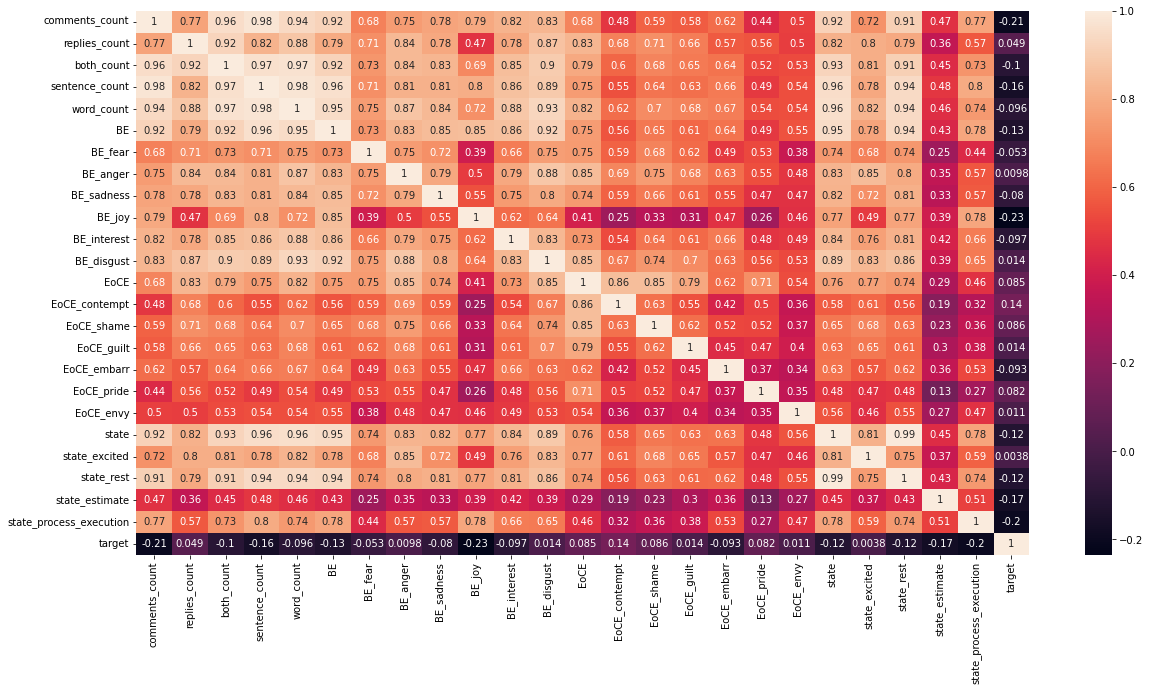
\includegraphics[width=\textwidth]{corr1.png}\newline\noindent
\end{center}
Видно, что некоторые признаки почти полностью линейно зависят от других. Это не удивительно: чем больше слов написал пользователь, тем больше предложений и самих комментариев. Удаляю все признаки, для которых коэффициент корреляции $R \ge 0.9$: \texttt{both\_count}, \texttt{sentence\_count}, \texttt{word\_cound}, \texttt{BE}, \texttt{state}, \texttt{state\_rest}.
\pagebreak

Теперь матрица корреляции выглядит так:
\begin{center}
      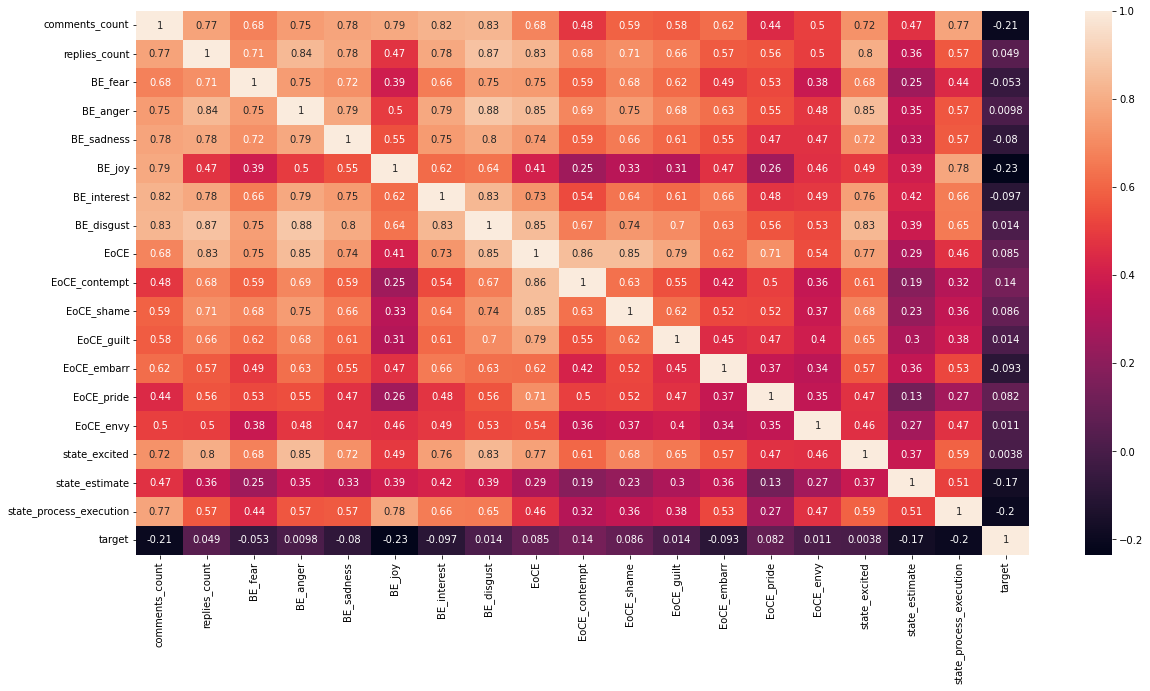
\includegraphics[width=\textwidth]{corr2.png}\newline\noindent
\end{center}
Классы \texttt{target} сильно не сбалансированы, поэтому я случайно удаляю классы $1$ и $2$ так, чтобы всех классов было поровну:
\begin{lstlisting}[language=python, keepspaces=true]
COEF_UNDER = 1
CLASSES = 2

ds_0 = ds[ds["target"] == 0]
ds_other = ds[ds["target"] != 0]
down_ds_other = ds_other.sample(n=len(ds_0) * CLASSES * COEF_UNDER, random_state=1)
ds = pd.concat([down_ds_other, ds_0])
\end{lstlisting}
Нормализую все признаки, чтобы они были в промежутке $[0, 1]$.
\begin{lstlisting}[language=python, keepspaces=true]
X = normalize(X, norm="max", axis=0)
\end{lstlisting}
Разбиваю данные на обучающую и тестовую выборку в соотношении 80 к 20.
\begin{lstlisting}[language=python, keepspaces=true]
train_X, test_X, train_y, test_y = train_test_split(
      X, y, train_size=0.8, random_state=1, shuffle=True
)
\end{lstlisting}
\pagebreak